\documentclass[fontsize=11pt]{article}
\usepackage{amsmath}
\usepackage{hanging}
\usepackage{xurl}
\usepackage[utf8]{inputenc}
\usepackage[margin=0.75in]{geometry}
\usepackage{graphicx}
\graphicspath{ {./images/} }

\title{CSC110 Project Report: Climate Change and its Scorching Effects on California}
\author{Andy Wang}
\date{\today}

\begin{document}
\maketitle

\section*{Problem Description and Research Question}
California has always been the target of severe wildfires, due to their hot, dry climate (Pierre-Louis, 2020). In fact, California's fire record dates all the way back to 1932 - a testament to their perpetually warm and dry climate (Pierre-Louis, 2020). Obviously, severe wildfires pose a huge threat; they can cause mass destruction and property damage, loss of life (human and animals), and most severely, the loss of trees and forests.

Loss of life and building damage isn't the only harmful outcome of these fires. The smoke that comes from fires can be scarring and irreparable, too. As fires scorch forests, clouds of smoke and carbon plague the air, which can have lasting effects on the climate such as interfering with rays from the sun (Brown, 2017). This smoke can travel in clouds, spreading itself far from the source (Brown, 2017). Inhalation of this smoke comes with many consequences, like irritation, difficulty breathing (like shortness of breath), worsening asthma and heart disease, and decreasing the body's oxygen supply (health.ny.gov).

So of course, the main motivation for choosing this as my topic is to spread awareness on the issue at hand. The issue is made even more concerning given the fact that climate change exists, and temperatures are on the rise. In fact, in the last century the temperature of California has risen by 3 degrees Fahrenheit, and heat waves are becoming more common (EPA, 2016). This is concerning because as mentioned before, hot equals fire, and the hotter it gets, the more fires there will be, and the more disastrous the effects will be.

This is why I chose my question to be: \textbf{how has the increase in California's temperature affected the severity (number of fires and acreage burned) of California's
annually wildfire seasons?} Answering this by analyzing data on past wildfire seasons will provide us with insight into the effects on climate change, and by extrapolating current trends, we can either prepare ourselves for what's to come, or can start taking preventative measures.

\section*{Dataset Description}
I could not find a single, downloadable dataset. Instead, I was able to find multiple PDF reports from \url{https://www.fire.ca.gov/stats-events/} from 2008 to 2020, which had the information I needed, so I just used those to compile the information. Some information about 2019 and 2020 were missing, so I filled them in from these websites:\\

\url{https://www.mercurynews.com/2019/11/05/map-californias-five-biggest-fires-this-season-plus-comparing-kincade-to-san-jose/}\\

\url{https://www.sacbee.com/news/california/fires/article245917915.html}\\

The data I took was that which I found most important, which is each season's year, total number of fires, total acreage burned, and top five individual fires. For each individual fire, I took the county it took place in, acreage burned, the cause, and the structures destroyed. These are all used by my program.

The dataset I cobbled together is in a \texttt{.txt} file, and is in the following format:
\begin{center}
    year\\
    The next five lines are: county, acreage, cause, structures destroyed, representing the season's top five fires\\
    total \# of fires, acreage of the season
\end{center}
And it repeats for each season.

\section*{Computational Overview}

To give a brief overview: my program reads through a text file, converts the text into data, computes on that data, and visualizes it.\\

When first run, my program calls the function \texttt{get\_fire\_data} on the file \texttt{cali\_fire\_data.txt}. This functions goes through the file, parses each line to find each individual attribute (like number of fires and acreage), and creates \texttt{CaliFire} and \texttt{CaliFireSeason} objects to store these attributes. It also aggregates a dictionary that maps a year to its corresponding fire season, and returns it.\\

It then calls the function \texttt{predict\_fire\_season\_data} with the dictionary, which uses the linear regression model to extrapolate the number of fires and total acreage of future fire seasons. It also predicts the top five fires of that season with an algorithm that makes use of \texttt{random.choice}: it aggregates a list containing all of the top five fires of all the seasons in the dataset, with duplicates allowed. Then to pick the next top five counties, it chooses five counties randomly. Since duplicates are allowed, this means that counties that appear more often in the list will be more vulnerable, and thus are more likely to be picked.

It also aggregates a dictionary mapping counties to lists of causes. So for example, if three fires in Los Angeles started due to lightning, and one to arson, then the dictionary entry for Los Angeles will look like: \texttt{[Lightning, Lightning, Lightning, Arson]}. The algorithm takes the five counties that it chose, and randomly assigns each county a cause from its respective dictionary entry. So if Los Angeles was chosen, then it is very likely that a fire would be caused by lightning.

Using the number of fires, acreage, and top five fires, it mutates the original dictionary by adding new entries. These entries start at year 2021, and are predictions for the future.\\

My program then runs another algorithm (a while loop) to initiate pygame and visualize the data. It calls the function \texttt{display\_season\_data} on the dictionary of seasons to draw the graph on top of the screen using a for loop. I also created a \texttt{ScrollableObject} class which represents objects that can be drawn on the screen and scrolled. I populate a list of these every time the user presses the left or right arrow keys and draw them using the \texttt{draw\_scrollables} function.

In addition, there is a helper function \texttt{get\_counties\_on\_map} which takes the top five fires of a season and makes \texttt{ScrollableObject} instances of them. Sometimes a county has multiple fires that make it to the top five, so this function aggregates these as well. Visually, these fires are represented by circles on map. My algorithm keeps track of the user's mouse coordinates and repeatedly checks to see if the mouse is hovering over one of these circles. If this is happening, then it calls the \texttt{display\_county\_fire\_info} to display the county's info about fires. The algorithm also checks to see if the user is scrolling, and calls the \texttt{scroll\_objects} to scroll all the scrollable objects up or down.\\

Obviously, I chose to use pygame to a greater extent than seen in class in order to meet the technical requirements. It has all I need to represent data in a visual and interactive way. In class, all that was shown with pygame was a few simple shapes, with a little bit of button input - like the spinning wheel and the convex hull visualization. My program uses pygame to a greater extent largely because it draws more complicated things, and it even uses object-oriented programming to keep track of the coordinates of these objects. It also incorporates more mouse interaction, such as scrolling.

\section*{Dataset and Program Instructions}
The dataset is relatively small, so I just included it in the MarkUs submissions. It should be called \texttt{cali\_fire\_data.txt}, and it should be put in the same directory as \texttt{main.py}. Do note that there are three images: \texttt{circle\_info.PNG}, \texttt{window.PNG}, and \texttt{county\_map.JPG}. The map is used by the program, and the other two are used for the PDF. 

All you need to do is run the file, and a screen should appear:

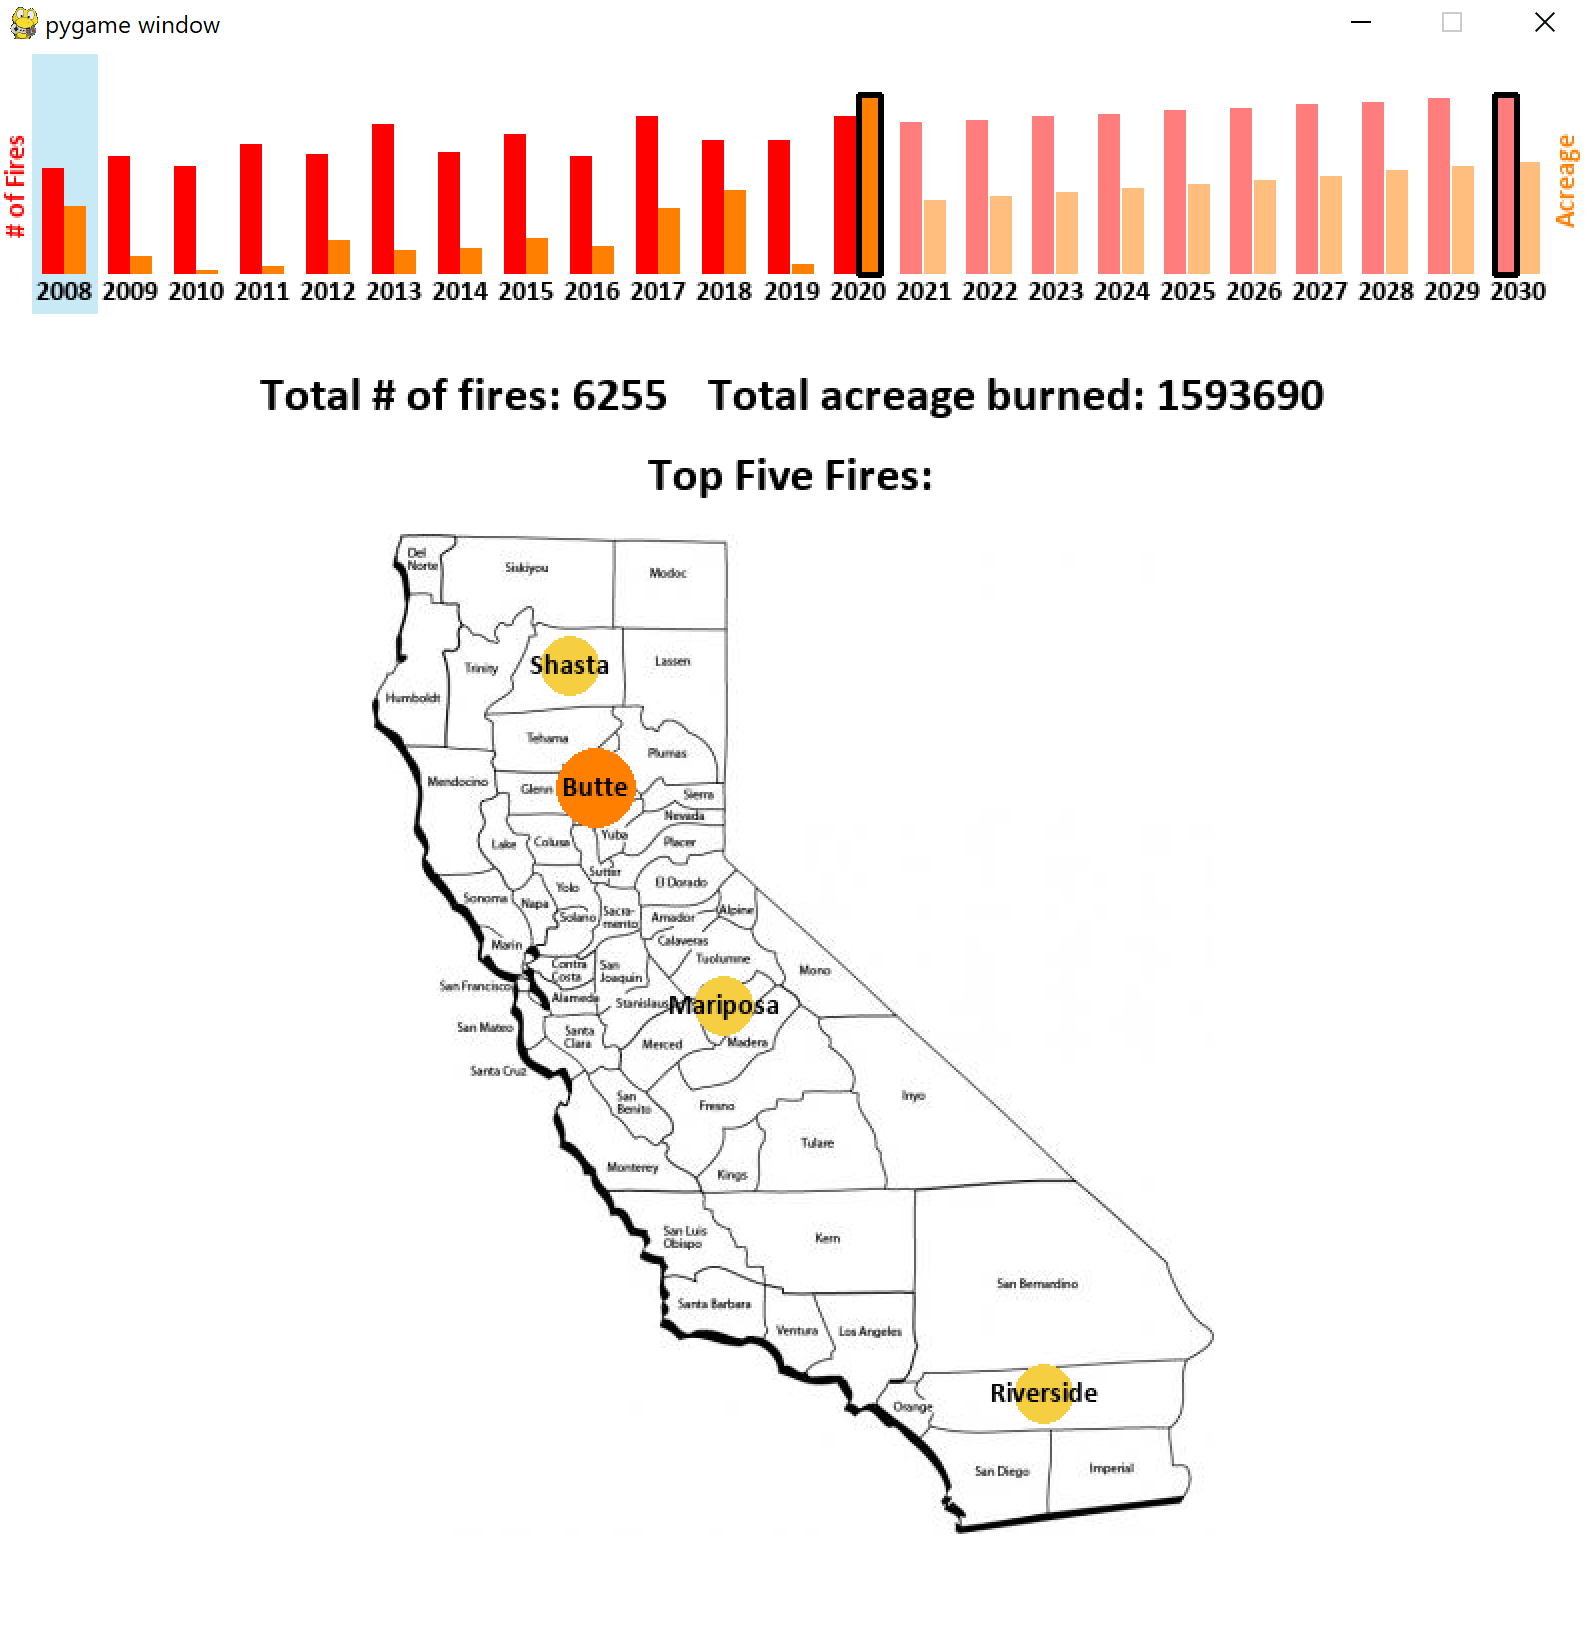
\includegraphics[scale=0.5]{window.PNG}

The graph on the top represents the fire season data. The entries past 2020 are extrapolated using the line of best fit found from linear regression. The red bars represent the number of fires, and the orange bars represent the acreage burned. Do note however that the bars are not proportional to each other, but are proportional to the maximum value of each data. That is to say, just because a red bar is higher than the orange one, does not mean that the number of fires exceeds the acreage - it just means that the number of fires is closer to the maximum number of fires in the data than the acreage is to the maximum acreage. Speaking of maximums, the maximum number of fires and acreage are shown by a black outline around the bar.

You can see a light blue box surrounding a pair of bars on the top - this represents what season you are currently looking at. You can press the left and right arrow keys to change what seasons you're looking at, and it even wraps around to! So if you go to 2030 and press right, you'll end up back at 2008.

The map of California shows the top five fires of the season. The redder and larger the circle, the more severe the fire is. You can hover your mouse over the circles to see info about each fire. Do note however that multiple fires can happen at the same county, and this is reflected when you hover your mouse over a circle:

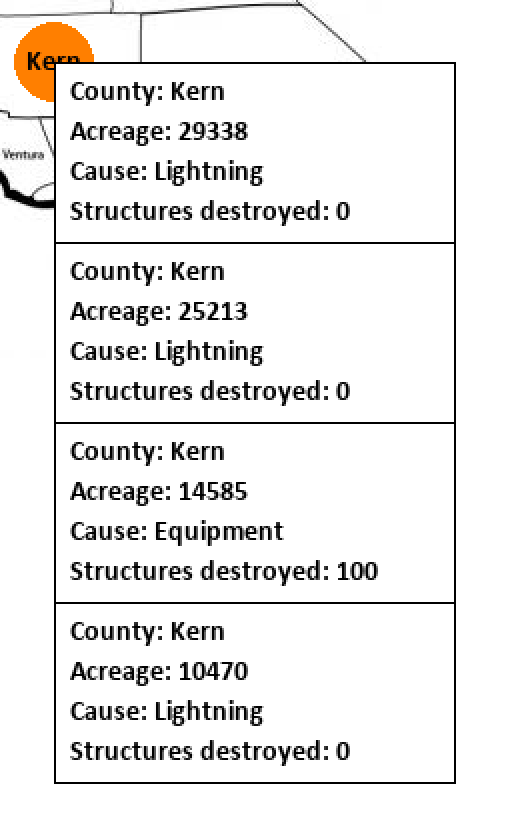
\includegraphics[scale=0.6]{circle_info.PNG}

I also added the ability to scroll the image up and down, in case any of the fire's info appears outside of the window. You can exit the program by clicking the window's X button or by pressing escape on your keyboard.

\section*{Changes to Proposal}
My previous idea was about Australian bushfires instead of California. But I couldn't find any reliable datasets on that, and a TA said that the dataset I was able to put together was "concerning" because I rounded too much. This is the main reason why I switched to California, because as explained in my dataset description, I was able to find reliable, concrete data and information.

I was not, however, able to find a graph or data showing the change in California's annual temperature. All I could find was that it increased by 3 degrees Fahrenheit, and that was it. Concrete data about the temperature would have been ideal because then I could have compared the temperature graph to the fire graph, leading to a visual representation of the correlation between temperature and fire.

The best I could do was just to just tell you that the temperature is rising, and show you the fire graph only. It was either this, or use inaccurate Australian fire data.

It is also worth noting that an important piece of data I added was location data. Previously I was planning on drawing random orange circles all over Australia, and these would get bigger and redder the more severe a bushfire season was. But following TA feedback, I was able to get concrete location data for California, and will draw things based on this data.

\section*{Discussion}

The results of my computation definitely helped me solve my question. It is clear from the graph, and from the extrapolation of that graph, that fire seasons are getting more and more severe as California's temperature rises. The number of fires of each seasons is clearly increasing, and the total acreage burned in each season is too. Thus, my research question is solved: the increase in California's temperature has affected the severity of annual wildfire seasons greatly, as the number of fires and acreage burned have been steadily increasing over the past decade.\\

According to my program, the acreage burned peaks in 2020, and the number of fires peaks in about 2030. This implies that at the current rate, fire seasons will continue to get more severe at about a constant rate. According to the map, it seems that most of the more severe county fires tend to take place in the middle of California, which suggests that the middle is drier and hotter than the rest.\\

It is worth mentioning that my extrapolation may not be entirely accurate. One limitation I encountered was the relatively small size of my dataset. If I were able to get a hold of California's fire season record since 1932 (this is where California's record dates back to, as mentioned in the first section), my predictions could have been a lot more accurate. Perhaps the severity of the fire seasons does not grow linearly, and is instead growing exponentially. A larger dataset would reveal that, and I could use a different regression model to extrapolate from.

With a larger dataset I also could have had more information about individual county fires, and could predict the next top five fires more accurately. With my current dataset I did not have enough of this information, so when predicting individual county fires I had to leave out acreage.\\

In regards to next steps for further exploration, one could consider the land that the fires are burning. Are they burning in forests? Or cities? This could potentially affect the next fire season, because we need to consider what the next season will burn on in order to predict it. A fire may not spread as much in the city as it does in the forest. 

Another factor worth looking into is the weather. Fires tend to spread faster in droughts than in rain. Level of preparedness is also a major factor. The spread of fire can be greatly reduced by a good firefighting team and the quality of their equipment, and with advancements in meteorology and technology, the growth in severity of fire seasons may not be as quick as currently predicted.\\

In conclusion, the increasing severity of fire seasons offers great insight into the damaging effects of climate change. There is a clear correlation between temperature and the acreage burned of a wildfire - and if we do nothing about it, it is only going to get worse. This is why we need to be prepared | only with computation and statistics can we predict trends in climate change, and knowing what the circumstances are for us in the future, we can be motivated to take the necessary preventative measures.

\section*{References}
\begin{hangparas}{0.25in}{1}
Bay Area News Group. (2019, November 5). Map: California’s five biggest fires this season, plus comparing Kincade to San Jose. \emph{The Mercury News.} \url{https://www.mercurynews.com/2019/11/05/map-californias-five-biggest-fires-this-season-plus-comparing-kincade-to-san-jose/}\\

Brown, J., \& Atkinson, J. (2017, June 13). \emph{Smoke from wildfires can have lasting climate impact.} Nasa. \url{https://climate.nasa.gov/news/2597/}\\

California Government. (2020). \emph{Stats and Events.} \url{https://www.fire.ca.gov/stats-events/}\\

United States Environmental Protection Agency. (2016, August). \emph{What Climate Change Means for  California.} EPA. \url{https://www.epa.gov/sites/production/files/2016-09/documents/climate-change-ca.pdf}\\

McGough, M. (2020, September 22). 5 of the 6 largest California wildfires in history started in the past 6 weeks. \emph{The Sacramento Bee.} \url{https://www.sacbee.com/news/california/fires/article245917915.html}\\

New York Government. (2020, January). \emph{Exposure to Smoke from Fires}. \url{https://health.ny.gov/environmental/outdoors/air/smoke_from_fire.htm}\\

Pierre-Louis, K., \& Schwartz J. (2020, December 3). Why Does California Have So Many Wildfires? \emph{The New York Times.} \url{https://www.nytimes.com/article/why-does-california-have-wildfires.html}\\

Pygame Community. (2020). \emph{Pygame Documentation.} Pygame. \url{https://www.pygame.org/docs/}

% NOTE: LaTeX does have a built-in way of generating references automatically,
% but it's a bit tricky to use so we STRONGLY recommend writing your references
% manually, using a standard academic format like APA or MLA.
% (E.g., https://owl.purdue.edu/owl/research_and_citation/apa_style/apa_formatting_and_style_guide/general_format.html)
\end{hangparas}
\end{document}
